% !TEX root = ../1-main-SL.tex
% !TEX encoding = UTF-8  (utf8)

\begin{frame}
	\centering
	\bf\Huge\color{purple} 习题讲评\\[1em]
	\small 习题1-3 -- 习题1-5\\[1cm]
	\small\color{gray}2018-10-31
\end{frame}

\section{说在前面}

\begin{frame}[t]\frametitle{说在前面}
	\linespread{1.8}
	\Large
	\vspace*{-1em}
    \begin{itemize}
    	\item 作业订正
    	\begin{enumerate}
    		\item {\it\Large\baa 不订正一律C,新作业不予批改}
    		\item {\it\Large 尽量就近订正}
    	\end{enumerate}
    	\item 关于雷同
    	\begin{enumerate}
    		\item {\it\Large 不要太明显,抄也要动脑子!}
    		\item {\it\Large\baa 发现明显的抄袭,相关人一律C}
    	\end{enumerate}
    	\item 几个小问题
    	\begin{enumerate}
    		\item {\it\Large 无意义的极限,如:
    		$\limx0\df1x$,$\limx{\infty}\arctan x$}
    		\item {\it\Large 求渐近线一定要仔细,避免遗漏}
    		\item {\it\Large 作业和笔记不要写在同一个本子上!}
    	\end{enumerate}
    \end{itemize}
\end{frame}

\section{参考解答}

\subsection{习题1-3}

\begin{frame}[t]\frametitle{1.用极限的定义证明}
\large
(1)$\limx{-2}{x^2}=4$

证:\it 对任意$\e>0$,令$\delta=\min\left\{1,\frac{\e}5\right\}$,
则对任意$x\in U_0(-2,\delta)$,总有$|x+2|<5$,进而
$$|x^2-4|=|x-2||x+2|<5|x+2|<5\cdot\df{\e}5<\e,$$
由极限的定义,即证。\fin
\end{frame}

\begin{frame}[t]\frametitle{1.用极限的定义证明}
\large

(2)$\limx{+\infty}\df{\sin x}{\sqrt x}=0$.

证:\it 对任意$\e>0$,令$X=\df1{\e^2}$,则对任意$x>X$,总有
$$\left|\df{\sin x}{\sqrt x}-0\right|\leq\df1{\sqrt x}
<\df1{\sqrt X}=\e.$$
由函数极限的定义,即证。\fin
\end{frame}

\begin{frame}[t]\frametitle{1.用极限的定义证明}
\large

(3)$\limx{\infty}\df{x+\sin x}{x+\cos x}=1$.
\bs

证:\it 对任意$\e>0$,令$X=\sqrt2/\e-1$,则对任意$|x|>X$,总有
$$\left|\df{x+\sin x}{x+\cos x}-1\right|
=\df{|\sin x-\cos x|}{|x+\cos x|}
<\df{\sqrt2}{|x|-1}<\df{\sqrt2}{X-1}=\e,$$
由函数极限的定义,即证。\fin
\end{frame}

\begin{frame}[t]\frametitle{Dirichlet函数的极限}
\large

2.证明:$f(x)=xD(x)$仅当$x=0$时极限存在。($D(x)$表示Dirichlet函数)
\bs

证:\it 对任意$\e>0$,令$\delta=\e$,对任意$x\in U_0(0,\delta)$,
注意到$|D(x)|\leq 1$,故总有
$$|xD(x)-0|\leq |x|<\delta=\e,$$
由函数极限的定义,$\limx0f(x)=0$。
\end{frame}

\begin{frame}[t]\frametitle{Dirichlet函数的极限(续)}
\large
\it
以下证明对任意$x_0\ne 0$,$\limx{x_0}f(x)$不存在。

对任意$x_0\ne0$,总可以取一个有理数列$\{x_n^{(1)}\}$
和一个无理数列$\{x_n^{(2)}\}$,使得
$$\limn x_n^{(1)}=\limn x_n^{(2)}=x_0.$$
注意到
$$\limn f(x_n^{(1)})=\limn x_n^{(1)}=x_0
\ne 0=\limn f(x_n^{(2)}),$$
故由Henie定理可知,当$x\to x_0$时$f(x)=xD(x)$不收敛。\fin
\end{frame}

\subsection{习题1-4}

\begin{frame}[t]\frametitle{无界与无穷大}
\large
1.证明:函数$y=\df1x\sin\df1x$在区间$(0,1]$内无界,但不是$x\to0^+$
时的无穷大。

\bs
证:\it 先证该函数无界。对任意$M>0$,总可令$x_M=\df1{2([M]+1)\pi+\frac{\pi}2}$,
则
\begin{align*}
	y(x_M)&=\left(2([M]+1)\pi+\frac{\pi}2\right)
	\sin\left[2([M]+1)\pi+\frac{\pi}2\right]\\
	&=2([M]+1)\pi+\frac{\pi}2>M.
\end{align*}
由函数无界的定义,即证。
\end{frame}

\begin{frame}[t]\frametitle{无界与无穷大(续)}
\large
\it 下证该函数不是$x\to0^+$时的无穷大。用反证法,若该函数是$x\to0^+$时的
无穷大,则$\limx{0^+}\df1y=0$。
考虑数列$x_n=\frac1{n\pi}$,显然$\limn x_n=0$,且$\sin\df1{x_n}=0$,
进而可知$\limn y(x_n)=0$。于是由Henie定理:
\begin{align*}
	1&=\limn y(x_n)\df1{y(x_n)}
	=\limn y(x_n)\limn\df1{y(x_n)}\\
	&=\limn y(x_n)\limx{0^+}\df1{y(x)}=0,
\end{align*}
显然不成立,由此即知假设错误,即证。\fin
\end{frame}

\begin{frame}[t]\frametitle{渐近线}
\large
2.求函数$y=\df1{1-x^2}$的水平渐近线和铅直渐进线。

解:\it 因为$\limx{\infty}y(x)=0$,故$x=0$是$y=\df1{1-x^2}$的水平渐近线;

又因为$\limx{\pm1}\df1{y(x)}=\limx{\pm1}(1-x^2)=0$,
故$y=\pm1$是$y=\df1{1-x^2}$的铅直渐近线。\fin

\centering
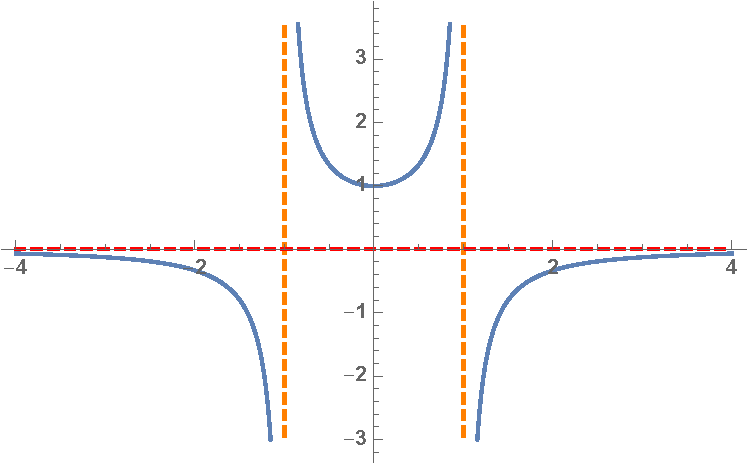
\includegraphics[width=0.6\textwidth]
{./images/ch01/11-x2.pdf}
\end{frame}

\subsection{习题1-5}

\begin{frame}[t]\frametitle{1. 计算如下极限}
\large
(1)
\begin{align*}
	\limx{1}&\left(\df1{1-x}-\df3{1-x^3}\right)
	=\limx1\df{(x-1)(x+2)}{(1-x)(1+x+x^2)}\\
	&=-\limx1\df{x+2}{1+x+x^2}=-1
\end{align*}

(2)
\begin{align*}
	\limx0&\df{(h+x)^3-h^3}x
	=\limx0\df{3h^2x+3hx^2+x^3}{x}\\
	&=\limx0(3h^2+3hx+x^2)=3h^2
\end{align*}
\end{frame}

\begin{frame}[t]\frametitle{1. 计算如下极限}
\large
(3)$\limx{\infty}\df{\arctan x}{x^2}$

解:{\it 因为$\limx{\infty}\df1{x^2}=0$,$|\arctan x|\leq\df{\pi}2$,
故由无穷小的性质可知:$\mbox{原式}=0.$}

\bs
(4)
\begin{align*}
	\limx{+\infty}&\df{\sqrt[3]{x+\sqrt{x+x^3}}}{\sqrt{x+1}}
	=\limx{+\infty}\df{\sqrt[3]{x^{-\frac12}
	+\sqrt{x^{-2}+1}}}{\sqrt{1+x^{-1}}}\\
	&=\df{\sqrt[3]{\limx{+\infty}x^{-\frac12}
	+\sqrt{\limx{+\infty}x^{-2}+1}}}{\sqrt{1+\limx{+\infty}x^{-1}}}=1.
\end{align*}
\end{frame}

\begin{frame}[t]\frametitle{1. 计算如下极限}
\large
(5)
\begin{align*}
	\limx4&\df{\sqrt{2x+1}-3}{\sqrt{x-2}-\sqrt2}
	=\limx4\df{(2x-8)(\sqrt{x-2}+\sqrt2)}{(x-4)(\sqrt{2x+1}+3)}
	=\df{2\sqrt2}3
\end{align*}

(6)
\begin{align*}
	\limx0&\df{\sqrt[3]{x+1}-1}x
	=\limx0\df{x}{x[(x+1)^{\frac{2}{3}}
	+(x+1)^{\frac{1}{3}}+1]}
	=\df13
\end{align*}
\end{frame}

\begin{frame}[t]\frametitle{1. 计算如下极限}
\large
(7)
\begin{align*}
	\limx0&\df{\sqrt{1+x}+\sqrt{1-x}-2}{x^2}
	=\limx0\df{2(\sqrt{1-x^2}-1)}
	{x^2(\sqrt{1+x}+\sqrt{1-x}+2)}\\
	&=\limx0\df{-2x^2}{x^2(\sqrt{1+x}+\sqrt{1-x}+2)
	(\sqrt{1-x^2}+1)}=-\df14.
\end{align*}

(8)
\begin{align*}
	\limx{+\infty}&\df{\ln(2+e^{3x})}{\ln(3+e^{2x})}
	=\limx{+\infty}
	\df{3x+\ln(2e^{-3x}+1)}{2x+\ln(3e^{-2x}+1)}\\
	&=\limx{+\infty}
	\df{3+\df1x\ln(2e^{-3x}+1)}{2+\df1x\ln(3e^{-2x}+1)}
	=\df32
\end{align*}
\end{frame}

\begin{frame}[t]\frametitle{1. 计算如下极限}
\large
(9)
\begin{align*}
	\limx{+\infty}&x(\sqrt{x^2+1}-x)
	=\limx{+\infty}\df{x(\sqrt{x^2+1}+x)}{x^2}=\df12
\end{align*}

\bs
(10)$\limx{-\infty}x(\sqrt{x^2+1}-x)$

解:{\it 因为
$$\limx{-\infty}\df1{x(\sqrt{x^2+1}-x)}
=\limx{-\infty}\df{1/x^2}{-\sqrt{1+x^{-2}}-1}=0,$$
故$x$和$\sqrt{x^2+1}-x$均为$x\to-\infty$时的
无穷大,从而可知该极限不存在。}
\end{frame}

\begin{frame}[t]\frametitle{1. 计算如下极限}
\large
(11)$\limx0x^2\sin\df1x$

解:{\it 因为$\limx0x^2=0$,$\left|\sin\df1x\right|\leq1$,由无穷小的性质,可知
$\mbox{原式}=0.$}
\end{frame}

\begin{frame}[t]\frametitle{利用极限的性质进行推导}
\large
2.确定常数$a,b$的值,使得
$\limx{\infty}\left(\df{x^2}{x+1}-ax-b\right)=0$。

解:\it
\begin{align*}
	0&=\limx{\infty}\left(\df{x^2}{x+1}-ax-b\right)\limx{\infty}\df1x
	=\limx{\infty}\df{\frac{x^2}{x+1}-ax-b}{x}\\
	&=\limx{\infty}\left(\df{x}{x+1}-a-\df bx\right)
	=1-a,
\end{align*}
故$a=1$,进而
\begin{align*}
	b&=\limx{\infty}\left(\df{x^2}{x+1}-x\right)
	=\limx{\infty}\df{-x}{x+1}=-1.
\end{align*}
\fin
\end{frame}

\begin{frame}
	\centering
	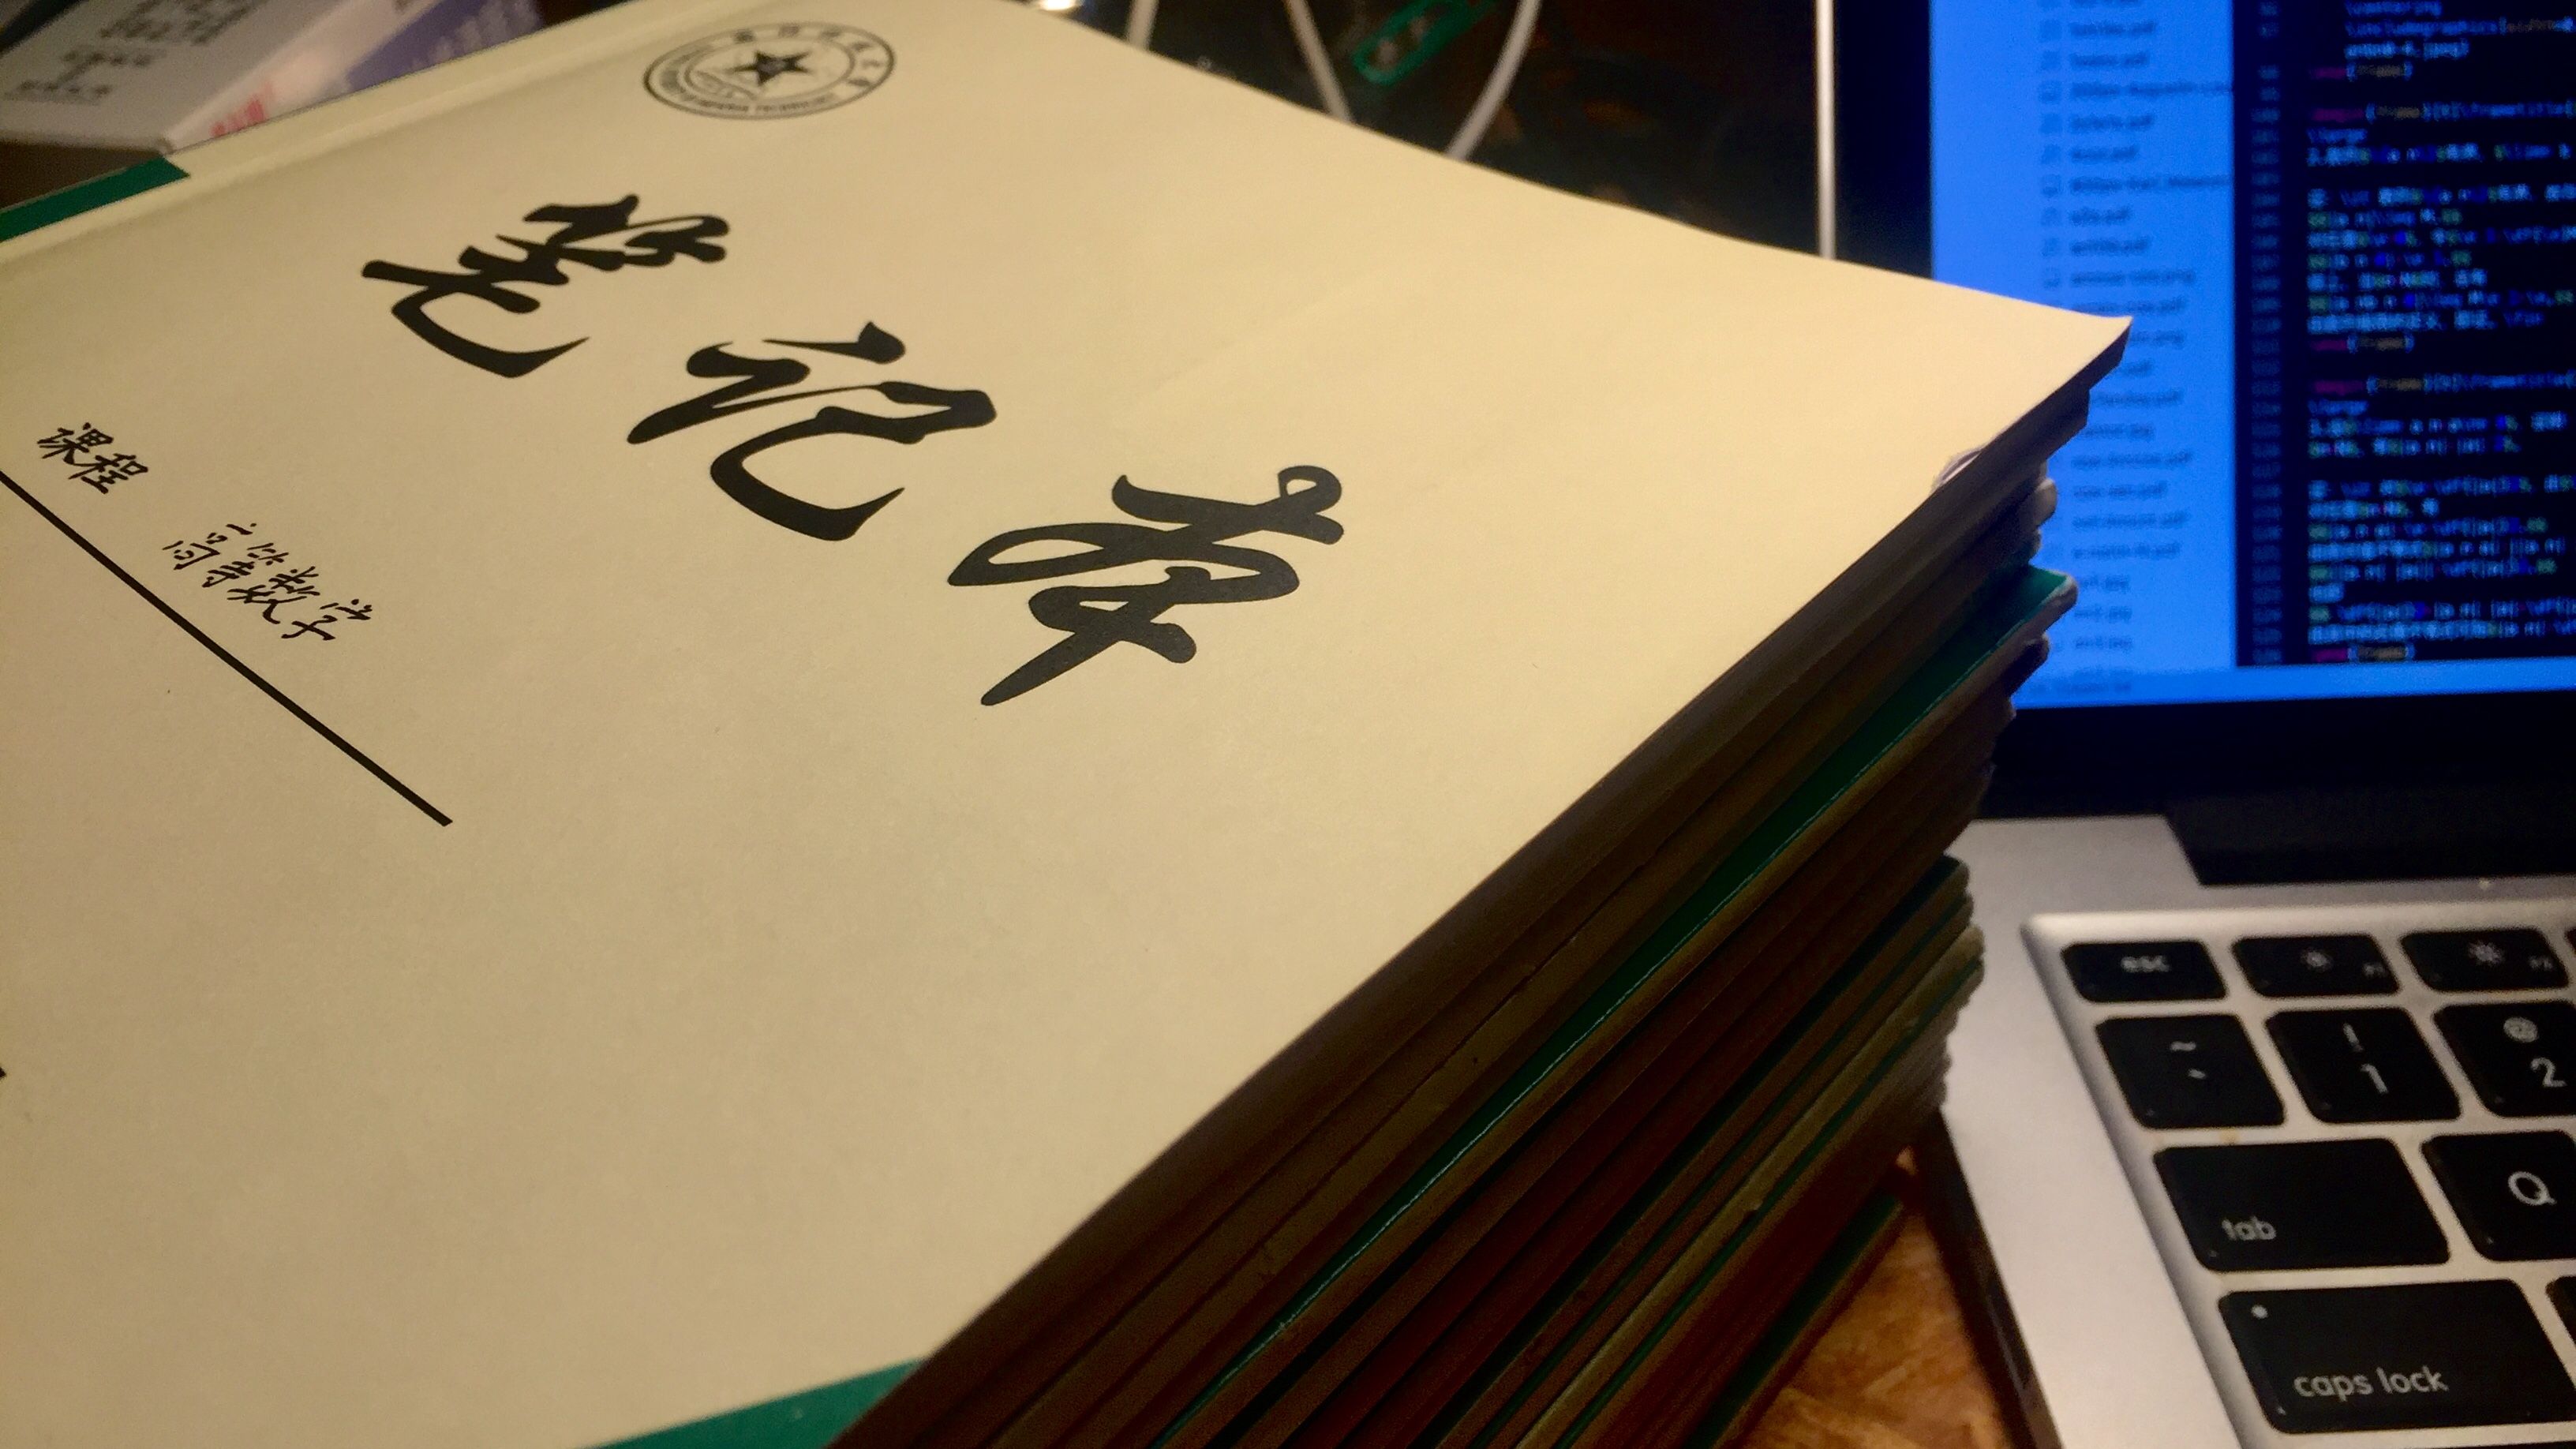
\includegraphics[width=\textwidth]{./images/ch01/HWR/notebook.jpg}

	\begin{flushright}
		\color{white}\vspace*{-2cm}
		\Huge\bf Q \& A
	\end{flushright}
\end{frame}